\documentclass{article}

\textwidth=6.5in
\textheight=8.5in
\voffset=-54pt
\oddsidemargin=0in
\evensidemargin=0in
\setlength{\parskip}{8pt}
\setlength{\parindent}{0pt}

\usepackage{amsmath, amssymb}
\usepackage{ifthen}

\usepackage[inline]{enumitem}
\setlist{topsep=0pt, parsep=8pt}

\usepackage[rgb,table]{xcolor}\convertcolorsUfalse
\usepackage{graphicx}

% change hyperref options
\PassOptionsToPackage{hyphens}{url}
\usepackage[bookmarks,colorlinks,linkcolor=black,citecolor=blue,pdfstartview=FitH,urlcolor=blue]{hyperref}
\hypersetup{pdfpagemode=UseNone}
\usepackage{bookmark}

\usepackage{graphicx}
\usepackage{multicol}
\usepackage{framed}
\usepackage{array}

\usepackage{icomma}

\usepackage{cancel}  

\usepackage{marginnote}
\usepackage[colorinlistoftodos]{todonotes}
\renewcommand{\marginpar}{\marginnote}

\usepackage{soul}
\usepackage[normalem]{ulem}

\usepackage{pgfplots}
\pgfplotsset{compat=1.18}  
\pgfplotscreateplotcyclelist{mycolor}{black, blue, red, green!70!black, magenta, purple, cyan, orange }  
\pgfplotsset{
  disabledatascaling,
  cycle list=tikzcolor, 
  axis lines=middle,
  every axis plot/.style={no marks, thick},
  every axis/.style={
    enlarge x limits=false,
    enlarge y limits=auto,
    xlabel style={at={(current axis.right of origin)},anchor=west},
    ylabel style={at={(current axis.above origin)},anchor=south},
    % extra x and y ticks for asymptotes
    extra x tick style={grid=major, grid style={dashed,black}},
    extra y tick style={grid=major, grid style={dashed,black}},
    /pgf/number format/1000 sep={},
  },    
  tick label style = {font=\footnotesize, fill=\currentbgcolor, inner sep=0pt},    
  xticklabel shift=1pt,    
  scaled ticks=false,
  scaled y ticks=false,
  unbounded coords=jump,
  samples=101,
  minor tick length=0,
  scatter/classes={
    open={mark=*,draw=black,fill=white, mark size=2, thin},
    closed={mark=*,draw=black,fill=black, mark size=2, thin}
  },
  width=3in,
}
\pgfplotsset{open/.style={only marks, mark=*, fill=white, thin, mark size=2}}
\pgfplotsset{closed/.style={only marks, mark=*, draw=black, fill=black,
    thin, mark size=2}}
\pgfplotsset{labeled/.style={nodes near coords, only marks, mark=*, draw=black, fill=black, thin, mark size=2, point meta=explicit symbolic}}

\usepackage{tikz}
\usetikzlibrary{
  matrix,%
  % enables the snake paths
  decorations.pathmorphing,%
  % enables bigger arrows
  decorations.markings,%
  decorations.pathreplacing,%
  decorations.text,%
  calc,%
  patterns,%
  shapes.geometric,%
  arrows,
  decorations.shapes,
  positioning,
  plotmarks,
  intersections,
  spy
}
\tikzset{>=latex} % sets default arrow type in tikz
\tikzset{font=\normalsize}
\tikzset{mark size=1.5pt, mark options=thin}
\tikzset{pin distance=4pt,
  every pin edge/.style={<-, thin, shorten <= -2pt}}

\interfootnotelinepenalty=10000
\renewcommand{\thefootnote}{(\arabic{footnote})}

\usepackage{multirow, bigdelim}

% change to \usepackage[sols]{handout} to see solutions
\usepackage[]{handout}

\newcommand\iscurrentenumi[1]{%
  \ifthenelse{\equal{#1}{\theenumi}}{}{#1}}
\setenumerate[1]{ref=\#\arabic*}
\setenumerate[2]{ref=\protect\iscurrentenumi{\theenumi}(\alph*)}
\newcommand\enumiiprefix[2]{%
  \ifthenelse{{\equal{#1}{\theenumi}}\AND{\equal{#2}{(\alph{enumii})}}}{}{}%
  \ifthenelse{{\equal{#1}{\theenumi}}\AND{\NOT{\equal{#2}{(\alph{enumii})}}}}{#2}{}%
  \ifthenelse{\equal{#1}{\theenumi}}{}{#1#2}%
}
\setenumerate[3]{ref=\protect\enumiiprefix{\theenumi}{(\alph{enumii})}\roman*}

\newlength{\tipmargin}
\makeatletter

\renewenvironment{framed}{
  \setlength{\tipmargin}{\textwidth-\linewidth}
  \advance\@totalleftmargin-\tipmargin
  \def\FrameCommand{\hspace{\tipmargin}\fbox}%
  \advance\linewidth\tipmargin
  \MakeFramed {\advance\hsize-\width \FrameRestore}%
}
{\endMakeFramed}

\makeatother

\definecolor{purple}{rgb}{0.5,0,1.0}

\usepackage{fancyhdr}
\lhead{\textcolor{white}{This content is protected and may not be shared, uploaded, or distributed.}}
\rhead{}
\rfoot{\vspace*{\fill}\footnotesize\textcopyright{} \emph{Harvard Math Ma}}
\renewcommand{\headrulewidth}{0pt}
\pagestyle{fancy}
\begin{document}

\htitle{Def\mbox{}inition and Interpretation of the Derivative}

\begin{problemonly}
  \begin{framed}

You should be able to:
    \begin{itemize}[topsep=0pt,partopsep=0pt,parsep=8pt,itemsep=0pt]
    \item State the definition of the derivative, explain where it comes from, and use it to calculate derivatives.

    \item Interpret the derivative in context and represent it graphically.

    \item Find the tangent line to the graph of $f(x)$ at $x = a$. 

    \item Use tangent lines to approximate function values, and determine whether such an approximation is too high or too low, or if there isn't enough information to be sure.
    \end{itemize}
  \end{framed}
\end{problemonly}

\begin{enumerate}
\item  \label{def-of-derivative}

  \note{This problem introduces the idea of the derivative. We'll do this together.}  

  A rocket is launched straight up into the air. Suppose the function $f(t) = t^2$ describes the rocket's height in meters $t$ seconds after liftoff.
  \begin{enumerate}
  \item \label{rocket-velocity-graph}

    \begin{problem}[2in]
      Sketch the graph of $f(t)$ for $t$ between 0 and 7. 
    \end{problem}

    \begin{solution}
    
      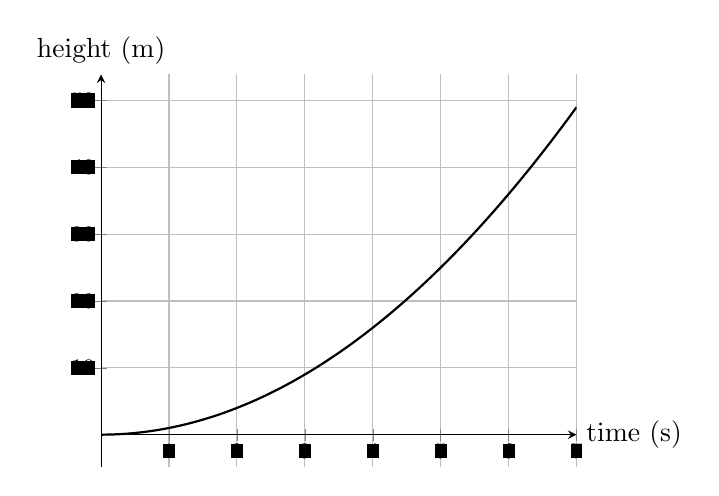
\begin{tikzpicture}
        \begin{axis}[xtick distance=1, grid=major, xlabel={time (s)}, ylabel={height (m)}]
          \addplot[domain=0:7]{x^2};
        \end{axis}
      \end{tikzpicture}
    \end{solution}

  \end{enumerate}
  Suppose you'd like to know the rocket's \emph{instantaneous} velocity $5$ seconds after liftoff. That is, you'd like to know how fast the rocket is going right at the instant $t = 5$.
  \begin{enumerate}[resume]
  \item
    \begin{problem}[0.35in]
      Would it work to find the rocket's average velocity between $t = 5$ and $t = 5$? Why or why not?
    \end{problem}

    \begin{solution}
      No, this would not work. If we tried to use the average rate of change formula,
      we would get an undefined expression:
      \[\frac{f(5)-f(5)}{5-5}=\frac{0}{0}.\]
    \end{solution}

  \item
    \begin{problem}[\vfill]
      How can we \emph{approximate} this instantaneous velocity? Write a general expression that \emph{approximates} the instantaneous velocity. How would you visualize your expression graphically?
    \end{problem}

    \begin{solution}
      One way to approximate the instantaneous velocity would be to find the average velocity between time $5$ and a time very close to $5$. If we let $x$ be our name for the time very close to $5$, this average velocity is $\displaystyle \frac{f(x) - f(5)}{x - 5}$, and we can visualize this as the slope of the secant line between $(5, f(5))$ and $(x, f(x))$ on the graph of $f(t) = t^2$.
      
      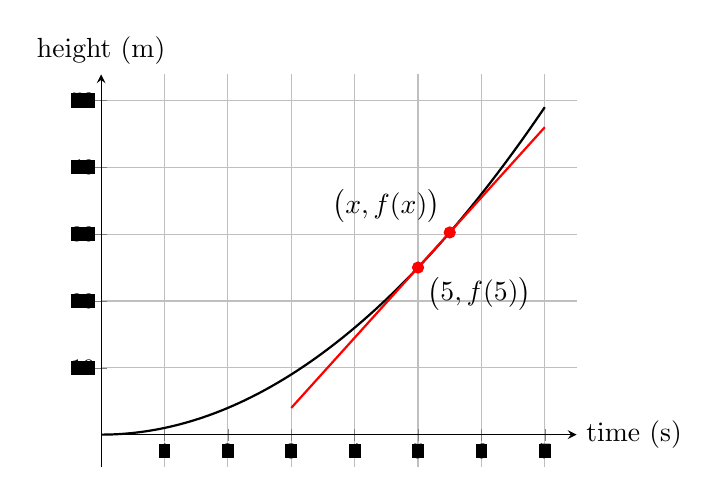
\begin{tikzpicture}
        \begin{axis}[xmax=7.5, xtick distance=1, grid=major, xlabel={time (s)}, ylabel={height (m)}]
          \addplot[domain=0:7]{x^2};
          \addplot[red, domain=3:7]{2*(5.5^2-5^2)*(x-5)+5^2};
          \addplot[closed, red] coordinates {(5,25) (5.5, 30.25)};
          \node[below right] at (5,25) {$\bigl(5, f(5)\bigr)$};
          \node[above left] at (5.5, 30.25) {$\bigl(x, f(x)\bigr)$};
        \end{axis}
      \end{tikzpicture}


      \emph{Alternate notation:} Instead of using $x$ to mean the time very close to $5$, we often write that time as $5 + h$ where $h$ is close to $0$. (For example, we could think of $5.01$ as $5 + 0.01$ or $4.99$ as $5 + (-0.01)$.) So, we could also think of finding the average velocity between times $5$ and $5 + h$, which is $\displaystyle \frac{f(5 + h) - f(5)}{(5 + h) - 5} = \frac{f(5 + h) - f(5)}{h}$, where $h$ is close to 0. Again, we can visualize this as the slope of the secant line between $(5, f(5))$ and $(5 + h, f(5 + h))$ on the graph of $f(t) = t^2$.

      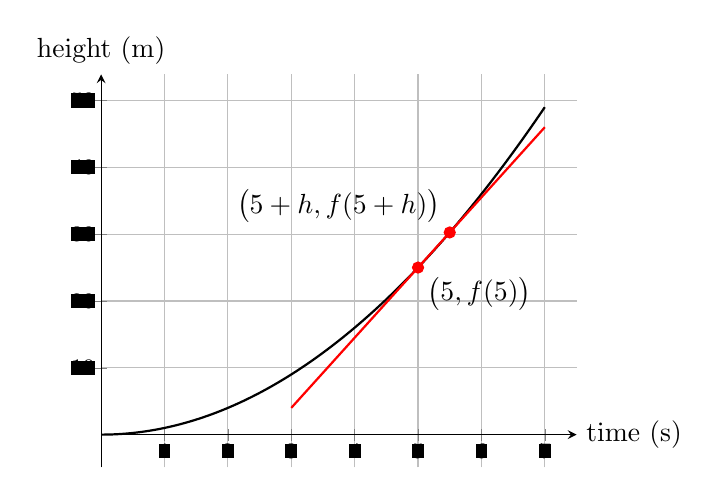
\begin{tikzpicture}
        \begin{axis}[xmax=7.5, xtick distance=1, grid=major, xlabel={time (s)}, ylabel={height (m)}]
          \addplot[domain=0:7]{x^2};
          \addplot[red, domain=3:7]{2*(5.5^2-5^2)*(x-5)+5^2};
          \addplot[closed, red] coordinates {(5,25) (5.5, 30.25)};
          \node[below right] at (5,25) {$\bigl(5, f(5)\bigr)$};
          \node[above left] at (5.5, 30.25) {$\bigl(5+h, f(5+h)\bigr)$};
        \end{axis}
      \end{tikzpicture}
    \end{solution}

  \item \label{rocket-velocity-find-and-visualize}

    \note{Here, I'll introduce the notation of limits. \url{https://www.geogebra.org/m/hnstunse} may be helpful for visualizing what happens as you let $h \to 0$.}

    \begin{problem}[\vfill]
      How could we find this instantaneous velocity \emph{exactly}? How would you visualize this instantaneous velocity graphically?
    \end{problem}

    \begin{solution} 
      To get the instantaneous velocity exactly, we'd like to find the
      average velocity between time $5$ and time $x$ when $x$ is as close
      to $5$ as possible.  Of course, it's not possible to pick a value of
      $x$ that is ``as close to $5$ as possible,'' but using a limit gives
      us what we want: the instantaneous velocity is exactly
      $\displaystyle \lim_{x \to 5} \frac{f(x) - f(5)}{x - 5}$.  We can
      visualize this as the slope of the tangent line to the graph of
      $f(t)$ at $t = 5$.

      \emph{Alternate notation:} If we instead write ``a time very close
      to $5$'' as $5 + h$, then we want $h$ to be ``as close to $0$ as
      possible''.  So, another limit that gives the instantaneous velocity
      is $\displaystyle \lim_{h \to 0} \frac{f(5 + h) - f(5)}{h}$.

      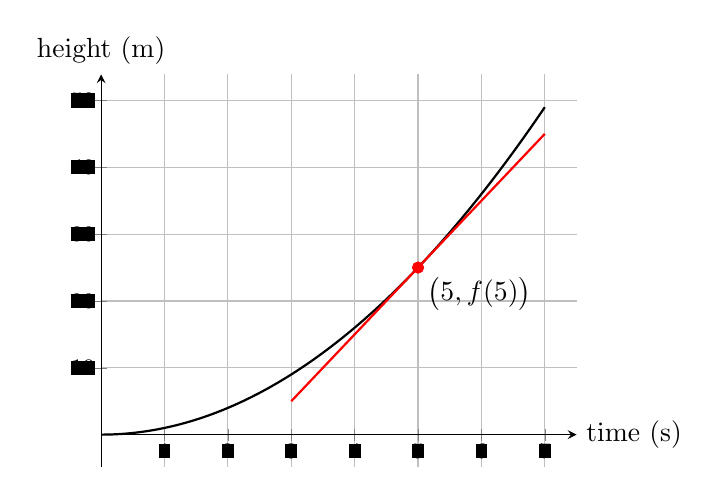
\begin{tikzpicture}
        \begin{axis}[xmax=7.5, xtick distance=1, grid=major, xlabel={time (s)}, ylabel={height (m)}]
          \addplot[domain=0:7]{x^2};
          \addplot[red, domain=3:7]{10*(x-5)+5^2};
          \addplot[closed, red] coordinates {(5,25)};
          \node[below right] at (5,25) {$\bigl(5, f(5)\bigr)$};
        \end{axis}
      \end{tikzpicture}
    \end{solution}

  \end{enumerate}
\end{enumerate}
\pspace{\newpage}

\probonly{
  \begin{framed}
    \textbf{Definition and interpretation of the derivative.}
    If we have a function $f(x)$ and a number $a$, we define the
    \uline{derivative of $f$ at $a$}, written $f'(a)$, to be
    \begin{center}
      $f'(a) = {}$ \fbox{
        \begin{minipage}{2in}
          \vspace{0.45in}\hspace{2.25in}
        \end{minipage}
      }
      \quad or \quad
      \fbox{
        \begin{minipage}{2in}
          \vspace{0.45in}\hspace{2.25in}
        \end{minipage}
      }
    \end{center}
    We read $f'(a)$ as ``$f$ prime of $a$.''
    \begin{itemize}
    \item We interpret $f'(a)$ as the instantaneous rate of change
      of $f$ at $x = a$.
    \item We visualize $f'(a)$ as the slope of the line tangent to the graph of $f$ at $x = a$.
    \end{itemize}
  \end{framed}
}

\begin{enumerate}[resume]
% \newpage

\item  \label{1/x-derivative}
  Let $\displaystyle f(x) = \frac{1}{x}$.
  \begin{enumerate}

  \item \label{1/x-derivative-graph}
    \begin{problem}[\stretch{3}]
      Sketch the graph of $f(x)$.  Sketch a line on your graph whose slope
      is $f'(1)$.  Based on this, is $f'(1)$ positive or negative?
    \end{problem}

    \begin{solution}
      The graph of $f(x)$ should be very familiar to you; here it is (in
      black), along with the line tangent to the graph at $x = 1$ (in
      blue), which has slope $f'(1)$:
      \begin{center}
        \begin{tikzpicture}
          \begin{axis}[ymin=-3.5, ymax=3.5, width=2.5in, height=2.5in,
            xtick={-2, 2}, ytick={-2, 2}, cycle list name=mycolor]
            \addplot+[domain=-3.5:3.5] {1/x};
            \addplot+[domain=-0.5:2.5] {-(x-1)+1};
          \end{axis}
        \end{tikzpicture}
      \end{center}
      This line has negative slope, so $f'(1)$ is \fbox{negative}. 
    \end{solution}

  \item

    \note{If \ref{def-of-derivative} takes longer than expected, I will skip this and the next part.}

    \begin{problem}[\vfill]
      Do you expect $f'(2)$ to be positive or negative? Is it greater than, less than, or equal to $f'(1)$?
    \end{problem}

    \begin{solution}
      On the graph, we can draw the line tangent to the graph at $x=2$ (in red) and compare
      its slope, $f'(2)$, to $f'(1)$.
      \begin{center}
        \begin{tikzpicture}
          \begin{axis}[ymin=-3.5, ymax=3.5, width=2.5in, height=2.5in,
            xtick={-2, 2}, ytick={-2, 2}, cycle list name=mycolor]
            \addplot+[domain=-3.5:3.5] {1/x};
            \addplot+[domain=-0.5:2.5] {-(x-1)+1};
            \addplot+[domain=0.5:3.5] {-0.25*(x-2)+1/2};
          \end{axis}
        \end{tikzpicture}
      \end{center}
      The red line has a negative slope, so $f'(2)$ is \fbox{negative.} The slope
      is less steep than the slope of the blue line, so $f'(2)$ is less negative than
      $f'(1)$. This means \fbox{$f'(2)>f'(1)$.}
    \end{solution}

  \item
    \begin{problem}[\vfill\newpage]
      Do you expect $f'(-2)$ to be positive or negative? Is it greater than, less than, or equal to $f'(2)$?
    \end{problem}

    \begin{solution}
      We can draw the lines which are tangent to the graph at $x=-2$ and $x=2$ and compare
      their slopes.
      \begin{center}
        \begin{tikzpicture}
          \begin{axis}[ymin=-3.5, ymax=3.5, width=2.5in, height=2.5in,
            xtick={-2, 2}, ytick={-2, 2}, cycle list name=mycolor]
            \addplot+[domain=-3.5:3.5] {1/x};
            \addplot+[domain=-3.5:-0.5] {-0.25*(x+2)-1/2};
            \addplot+[domain=0.5:3.5] {-0.25*(x-2)+1/2};
          \end{axis}
        \end{tikzpicture}
      \end{center}
      We can see that the slope of the tangent line that intersect the graph at $x=-2$ is
      negative, so $f'(-2)$ is \fbox{negative.} Because of the symmetry of the graph ($f$ is
      an odd function), the slopes of the two tangent lines are equal. Thus, \fbox{$f'(-2)=
      f'(2)$.}
    \end{solution}

  \item \label{1/x-derivative-calculate-derivative}
    \begin{problem}[\vfill]
      Calculate $f'(1)$ exactly using the definition of the derivative. Is this consistent with your answer to \ref{1/x-derivative-graph}?
    \end{problem}

    \begin{solution}
      \begin{align*}
        f'(1) &= \lim_{h \to 0} \frac{f(1 + h) - f(1)}{h} \\
        &= \lim_{h \to 0} \frac{\frac{1}{1 + h} - 1}{h} \\
        &= \lim_{h \to 0} \frac{\frac{1 - (1 + h)}{1 + h}}{h} \\
        &= \lim_{h \to 0} \frac{-\cancel{h}}{(1 + h) \cancel{h}} \\
        &= \lim_{h \to 0} \frac{-1}{(1 + h)} \\
        &= - 1
      \end{align*}
      As we expected from \ref{1/x-derivative-graph}, $f'(1)$ is indeed negative.
    \end{solution}

  \item

    \note{Encourage students to use point-slope form!}

    \begin{problem}[\nstretch{0.5}]
      Find the equation of the line tangent to $y = \dfrac{1}{x}$ at $x =
      1$. 
    \end{problem}

    \begin{solution}
      In \ref{1/x-derivative}, we found that the slope of this tangent line
      is $- 1$, so we just need to know a point on the tangent
      line.  Fortunately, we do: the line must include the point $(1, 1)$, so its equation is $\boxed{y - 1 = -(x-1)}$.
    \end{solution}

  \end{enumerate}

\item  \label{linear-approximation-turkey}
  % This is based on numbers from SPU27, in which they estimate that a
  % turkey which starts at 20 degrees in a 163 degree C oven has
  % temperature given by 163 - 143*E^(-t/8.65), where t is in hours

  \note{The goal of this problem is for students to see that, if we know a derivative, the the natural approximation we would make is exactly the tangent line approximation.

    This makes sense with what we saw visually in \ref{rocket-velocity-find-and-visualize}; when you zoom in on the graph around a point, it looks just like it's tangent line. (Of course, this is only true if the function is differentiable / locally linear there, but I won't bring this up unless students do; we'll talk more about this next time.)}

  Peter is roasting a 14 lb turkey as a test run for Thanksgiving. He starts roasting the turkey at noon. At 1:00pm, he checks on the turkey using a fancy thermometer; he discovers that it has an internal temperature of $35.6^\circ$C,\footnote{According to the USDA, a turkey should be roasted to an internal temperature of $73^\circ$C.} and its temperature is rising at an instantaneous rate of $0.25^\circ$C per minute.

  \begin{enumerate}
  \item \label{linear-approximation-turkey-approx}
    \begin{problem}[\vfill]
      Approximate the temperature of the turkey at 1:06pm.
    \end{problem}

    \begin{solution}
      The temperature of the turkey at 1:00 pm is $35.6^\circ$C. If we assume that the temperature continues rising at $0.25^\circ$C per minute for the next 6 minutes, then the turkey's temperature will be $35.6^\circ + (0.25^\circ / \text{minutes})(6 \text{ minutes}) = \boxed{37.1^\circ\text{C}}$ at 1:06 pm. (This is only an approximation because the turkey's temperature probably doesn't rise at a constant rate.)
    \end{solution}

  \item
    \begin{problem}[\vfill]
      Let $I(t)$ be the turkey's internal temperature (in $^\circ$C) $t$ minutes after noon. Use function notation to express what you were told about the turkey.
    \end{problem}

    \begin{solution}
      We were told that $I(60) = 35.6$ and $I'(60) = 0.25$. 
    \end{solution}

  \item

    \note{This is the last part I definitely want to do today (although I hope we will also have time to do the next 2 parts).}

    \begin{problem}
      Here is a graph of $I(t)$. Use a sketch to explain the approximation you made in \ref{linear-approximation-turkey-approx}.

      \begin{tikzpicture}
        \begin{axis}[xlabel=$t$, ylabel=$I$, xtick={60, 120, 180, 240},
          ytick=\empty, enlargelimits=false, ymin=0, width=2.75in] 
          \addplot+[domain=0:250] {163 - 143/e^(0.006289308176100629*x)};
        \end{axis}
      \end{tikzpicture}
    \end{problem}

    \begin{solution}
      In \ref{linear-approximation-turkey-approx}, we started with the fact that $I(60) = 35.6$ and assumed that the turkey's temperature would continue to rise at the \emph{constant} rate of $I'(60) = 0.25^\circ$C for the next 6 minutes; that is, we assumed that the turkey's temperature would change linearly. We were pretending that the graph of the turkey's temperature was a line including the point $(60, I(60))$ and having slope $I'(60)$. But this line is exactly the tangent line at $t = 60$. Here's a sketch:
      \begin{center}
        \begin{tikzpicture}
          \begin{axis}[xlabel=$t$, ylabel=$I$, xtick={60, 120, 180, 240},
            ytick=\empty, enlargelimits=false, ymin=0, width=2.75in, cycle
            list name=mycolor] 
            \addplot+[domain=0:250] {163 -
              143/e^(0.006289308176100629*x)};
            \addplot+[domain=20:120] { 0.616672 * (x - 60) + 65};
            \draw (50, 58.584) rectangle (70, 70.925);
            \coordinate (A) at (70, 58.584);
            \coordinate (B) at (70, 70.925);
          \end{axis}

          \draw (4, 1) rectangle (6, 3);
          \draw[thick] (4, 1) to [bend left=10] (6, 3);
          \draw[blue, thick] (4, 1.2) -- (5.8, 3);
          \draw (A) -- (4,1);
          \draw (B) -- (4,3);
          \draw (5.4,2.55) rectangle (5.6, 2.75);
          \draw (7, 2) rectangle (9, 4);
          \draw (5.6, 2.55) -- (7, 2);
          \draw (5.6, 2.75) -- (7, 4);
          \draw[thick] (7,2) -- (9,4);
          \draw[thick, blue] (7, 2.3) -- (8.5,4);
          \node[circle, fill=black, inner sep=1.5pt] at (8, 3) {};
          \node[yshift=-8pt, xshift=12pt] at (8, 3) {\tiny$(66,I(66))$};
          \node[circle, fill=blue, inner sep=1.5pt] at (8, 3.45) {};
          \node[yshift=8pt, xshift=-12pt, blue] at (8, 3.45) {\tiny$(66,37.1)$};
          \draw[thick, dotted] (8, 3) -- (8, 3.45);
          
        \end{tikzpicture}
      \end{center}
      Although what we wanted was the $y$-value on the black curve at $t = 66$, we approximated this by the $y$-value on the blue line at $t = 66$.
    \end{solution}

  \item \label{linear-approximation-turkey-approx-over-under}
    \begin{problem}[\vfill]
      Based on your sketch, was your approximation too high or too low? 
    \end{problem}

    \begin{solution}
      From our sketch, we can see that our approximation was \fbox{too high}.
    \end{solution}

  \item
    \begin{problem}[\vfill\newpage]
      Would you be comfortable using the same method to predict the turkey's temperature at 3 pm? Why or why not?
    \end{problem}

    \begin{solution}
      No. Although it seems pretty reasonable to say that the turkey's temperature changes at a roughly constant rate for 6 minutes, it seems pretty unlikely that it would change at a constant rate for 2 hours. Graphically, we can see that the tangent line is very close to the actual graph at 1:06 pm ($t = 66$), but it's not very close at 3:00 pm ($t = 180$):
      \begin{center}
        \begin{tikzpicture}
          \begin{axis}[xlabel=$t$, ylabel=$I$, xtick={60, 120, 180, 240},
            ytick=\empty, enlargelimits=false, ymin=0, width=2.75in, cycle
            list name=mycolor] 
            \addplot+[domain=0:250] {163 -
              143/e^(0.006289308176100629*x)};
            \addplot+[domain=20:240] { 0.616672 * (x - 60) + 65};
          \end{axis}
        \end{tikzpicture}
      \end{center}
    \end{solution}

  \end{enumerate}

\item  \emph{Practice interpreting notation.}

  Here's the graph of a function $f$.

  \pgfplotsset{
    /pgf/declare function={
      f(\x) = -atan(\x-4) + 150*e^(-(\x-5)^2/2);
      g(\x) = (f(\x+0.01)-f(\x))/0.01;}
  }

  \begin{center}
    \begin{tikzpicture}
      \begin{axis}[xtick={1, 2, ..., 8}, ytick=\empty, width=4in]
        \addplot+[domain=0:8.3] {f(x)}; 
      \end{axis}
    \end{tikzpicture}
  \end{center}

  In each part, you're given an expression. Sketch a line whose slope is the given expression.

  \begin{enumerate}
  \item
    \begin{problem}[\vfill]
      $\dfrac{f(6) - f(3)}{3}$
    \end{problem}

    \begin{solution}
    This is the slope of the secant line that intersects the graph at $x=3$ and $x=6$.
      \begin{center}
        \begin{tikzpicture}
          \begin{axis}[xtick={1, 2, ..., 8}, ytick=\empty]
            \addplot+[domain=0:8.3] {f(x)};
            \addplot[red,domain=0:8] {((f(6)-f(3))/3)*(x-3)+f(3)};          \addplot[closed, red] coordinates {(6,{f(6)}) (3,{f(3)})};  
          \end{axis}
        \end{tikzpicture}
      \end{center}
    \end{solution}

  \item
    \begin{problem}[\vfill]
      $\displaystyle \lim_{h \to 0} \dfrac{f(2 + h) - f(2)}{h}$ 
    \end{problem}

    \begin{solution}
    The value of this limit is the slope of the line tangent to the graph at $x=2$. 
      \begin{center}
        \begin{tikzpicture}
          \begin{axis}[xtick={1, 2, ..., 8}, ytick=\empty]
            \addplot+[domain=0:8.3] {f(x)};
            \addplot[red,domain=0:8] {g(2)*(x-2)+f(2)};
            \addplot[closed, red] coordinates {(2,{f(2)})};  
          \end{axis}
        \end{tikzpicture}
      \end{center}
    \end{solution}

  \item
    \begin{problem}[\vfill]
      $\displaystyle \lim_{w \to 3} \frac{f(w) - f(3)}{w - 3}$
    \end{problem}

    \begin{solution}
    This value of this limit is the slope of the line tangent to the graph at $x=3$. 
      \begin{center}
        \begin{tikzpicture}
          \begin{axis}[xtick={1, 2, ..., 8}, ytick=\empty]
            \addplot+[domain=0:8.3] {f(x)};
            \addplot[red,domain=0:7.5] {g(3)*(x-3)+f(3)};
            \addplot[closed, red] coordinates {(3,{f(3)})};  
          \end{axis}
        \end{tikzpicture}
      \end{center}
    \end{solution}

  \item
    \begin{problem}[\vfill]
      $\displaystyle \lim_{x \to 6} \frac{f(x) - f(4)}{x - 4}$
    \end{problem}

    \begin{solution}
    The value of this limit is $\dfrac{f(6)-f(4)}{6-4}$, which is the slope of the secant line
    that intersects the graph at $x=4$ and $x=6$.
      \begin{center}
        \begin{tikzpicture}
          \begin{axis}[xtick={1, 2, ..., 8}, ytick=\empty]
            \addplot+[domain=0:8.3] {f(x)};
            \addplot[red,domain=3.5:8] {((f(6)-f(4))/2)*(x-4)+f(4)};
            \addplot[closed, red] coordinates {(6,{f(6)}) (4,{f(4)})};  
          \end{axis}
        \end{tikzpicture}
      \end{center}
    \end{solution}

  \item
    \begin{problem}[\vfill]
      $\displaystyle \lim_{h \to 3} \frac{f(1 + h) - f(1)}{h}$
    \end{problem}

    \begin{solution}
    The value of this limit is $\dfrac{f(4)-f(1)}{3}$, which is the slope of the secant line that intersects the graph at $x=1$ and $x=4$.
      \begin{center}
        \begin{tikzpicture}
          \begin{axis}[xtick={1, 2, ..., 8}, ytick=\empty]
            \addplot+[domain=0:8.3] {f(x)};
            \addplot[red,domain=0:8] {((f(4)-f(1))/3)*(x-1)+f(1)};
            \addplot[closed, red] coordinates {(1,{f(1)}) (4,{f(4)})};  
          \end{axis}
        \end{tikzpicture}
      \end{center}
    \end{solution}

  \end{enumerate}

\end{enumerate}
\end{document}
